\section{TCAN Model}

% Reemplaza el frame "Problem Formulation" con este NUEVO frame combinado

\begin{frame}{TCAN Model}
\begin{columns}[T]
\column{0.85\textwidth}
\textbf{ \small Model Definition}
\begin{itemize}
    \item \scriptsize TCAN: Temporal Convolutional Attention Network.
    \item \scriptsize Feed-forward autoregressive model (each prediction becomes input for the next step).
    \item \scriptsize Controller in NFTM framework.
\end{itemize}

\textbf{\small Continuous Field}
\begin{itemize}
    \item \scriptsize $f_t$: snapshot of PDE solution.
    \item \scriptsize Vector of size $N$ (spatial positions).
    \item \scriptsize $f_t = [u(x_1,t), \ldots, u(x_N,t)]$.
    \item \scriptsize Shape: $(1 \times N)$.
\end{itemize}

\textbf{\small Input and Output of the Model}\\
\vspace{0.1cm}
\scriptsize To predict $f_{t+1}$, the corresponding input and output of the model are:
\begin{itemize}
    \item \scriptsize \textbf{Input}: \textbf{history window} (chunk of $W$ previous fields): $[f_{t - W + 1}, f_{t - W + 2}, ..., f_{t}]$ with size $(B, W, N)$.
    \item \scriptsize \textbf{Output}: \textbf{prediction of the field at next time step $t+1$}: $\hat{f}_{t+1}$, with size: $(B, 1, N)$.
\end{itemize}

\column{0.3\textwidth}
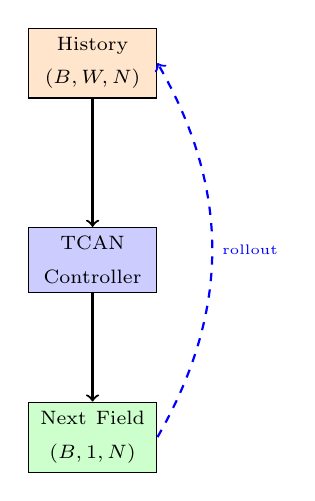
\begin{tikzpicture}[scale=0.25]

\node[rectangle, draw, fill=orange!20,
      text width=1.4cm, align=center,
      minimum height=0.65cm] 
(input) at (0, 15.5) {\scriptsize History\\$(B,W,N)$};

\node[rectangle, draw, fill=blue!20,
      text width=1.4cm, align=center,
      minimum height=0.65cm] 
(tcan) at (0, 5.5) {\scriptsize TCAN\\Controller};

\node[rectangle, draw, fill=green!20,
      text width=1.4cm, align=center,
      minimum height=0.65cm] 
(output) at (0, -3.5) {\scriptsize Next Field\\$(B,1,N)$};

\draw[->, thick] (input) -- (tcan);
\draw[->, thick] (tcan) -- (output);
\draw[->, thick, dashed, blue] (output.east)
      to[bend right=30] node[right, font=\tiny] {rollout} (input.east);

\end{tikzpicture}
\end{columns}
\end{frame}

\begin{frame}
\vspace{0.2cm}
\small \textbf{Autoregressive Roll-out Process}\\
\vspace{0.1cm}
\begin{itemize}
    \item \scriptsize Each TCAN call predicts next field from current window
    \item \scriptsize Window slides: drop oldest, add prediction
    \item \scriptsize Process repeats autoregressively for full trajectory
\end{itemize}
\scriptsize In the example below, the model first predicts $f_{21}$ from the window $[f_1,\dots,f_{20}]$, then uses the updated window $[f_2,\dots,f_{20},f_{21}]$ to predict $f_{22}$, and so on.
\vspace{0.2cm}

\begin{center}
\resizebox{0.3\textwidth}{!}{%
\begin{tikzpicture}[
    box/.style={draw, rectangle, rounded corners, minimum width=2.2cm, minimum height=0.8cm, align=center, fill=orange!20, font=\small},
    pred/.style={draw, rectangle, rounded corners, minimum width=1.6cm, minimum height=0.8cm, align=center, fill=green!20, font=\small},
    arrow/.style={->, thick, >=stealth},
    node distance=1.4cm
]

% Step 1
\node[box] (w1) {Window\\$[f_1,\dots,f_{20}]$};
\node[pred, right=of w1] (p21) {$\hat{f}_{21}$};
\node[font=\scriptsize, above=0.10cm of $(w1)!0.52!(p21)$] {TCAN};
\draw[arrow] (w1.east) -- (p21.west);

% Step 2
\node[box, below=of w1] (w2) {Window\\$[f_2,\dots,f_{20},\hat{f}_{21}]$};
\node[pred, right=of w2] (p22) {$\hat{f}_{22}$};
\node[font=\scriptsize, above=-0.55cm of $(w2)!0.55!(p22)$] {TCAN};
\draw[arrow] (w2.east) -- (p22.west);

% Step 3
\node[box, below=of w2] (w3) {Window\\$[f_3,\dots,f_{21},\hat{f}_{22}]$};
\node[pred, right=of w3] (p23) {$\hat{f}_{23}$};
\node[font=\scriptsize, above=-0.45cm of $(w3)!0.55!(p23)$] {TCAN};
\draw[arrow] (w3.east) -- (p23.west);

% Pred → next window (curvas por debajo, lejos del texto TCAN)
\draw[arrow] (p21.south) to[out=-60,in=20] (w2.north);
\draw[arrow] (p22.south) to[out=-60,in=20] (w3.north);

% Continuation dots
\node[font=\large] (dots) at ($(w3.south)!0.5!(p23.south) + (0,-1.2)$) {$\dots$};

\end{tikzpicture}%
}
\end{center}
\end{frame}

\begin{frame}
\small \textbf{TCAN Architecture}
\begin{columns}[T]
    \column{0.35\textwidth}
    \begin{center}
    \resizebox{1.25\textwidth}{!}{%
    \begin{tikzpicture}[
        box/.style={rectangle, draw, rounded corners, minimum width=2.4cm, minimum height=0.85cm, align=center, fill=blue!10},
        op/.style={rectangle, draw, rounded corners, minimum width=2.4cm, minimum height=0.85cm, align=center, fill=green!10},
        arrow/.style={->, thick, >=stealth},
        input/.style={rectangle, draw, rounded corners, minimum width=2.4cm, minimum height=1.0cm, align=center, fill=orange!20},
        output/.style={rectangle, draw, rounded corners, minimum width=2.4cm, minimum height=1.0cm, align=center, fill=red!20},
        node distance=2.0cm and 1.6cm
    ]
    % Main flow - left column
    \node[input] (input) {INPUT\\$f_{\text{history}}$};
    \node[op, below=of input] (embed) {Embedding\\Conv1d+GELU};
    \node[box, below=of embed] (features) {Features\\$(B,20,32,N)$};

    % Attention column - center-right
    \node[box, right=1.8cm of features] (query) {Query $Q$\\(last frame)};
    \node[op, below=of query] (attn) {Causal\\Attention};
    \node[box, below=of attn] (context) {Context\\$(B,32,N)$};

    % Decoder/output column - right
    \node[op, right=1.8cm of context] (decoder) {Decoder\\Conv1d};
    \node[box, below=of decoder] (corr) {Correction\\$\tanh(\times0.1)$};
    \node[output, below=of corr] (output) {OUTPUT \\$f_{\text{next}}$};

    % CLEAN ARROWS - NO CROSSING
    \draw[arrow] (input) -- (embed);
    \draw[arrow] (embed) -- (features);
    \draw[arrow] (features) -| ([xshift=-0.3cm]query.west) -- (query);
    \draw[arrow] (query) -- (attn);
    \draw[arrow] (attn) -- (context);
    \draw[arrow] (context) -- (decoder);
    \draw[arrow] (decoder) -- (corr);
    \draw[arrow] (corr) -- (output);

    % Residual from features to context (ABOVE)
    \draw[arrow, dashed, blue] (features.south) 
        to[out=-5,in=150] node[above, font=\footnotesize, black]{residual} 
        (context.west);

    % FIXED: LEFT→DOWN→RIGHT path from input to output
    \draw[arrow, dashed, orange, thick] (input.south) 
        |- ++(-2,0)     % LEFT (west)
        |- ++(0,-18)     % DOWN (south) 
        -| (output.west)     % RIGHT to output
        node[below, font=\scriptsize, pos=0.1]{$f_t$};


    % KV note
    \node[font=\footnotesize, align=center, right=0.2cm of query, anchor=west] (kv) {$K,V$\\all frames};
    \end{tikzpicture}%
    }
    \end{center}
    
    \column{0.6\textwidth}
    \begin{itemize}
      \item \scriptsize \textbf{$f_{\text{history}}$}: chunk of 20 previous fields, size: $(B,20,N)$.
      \item \scriptsize \textbf{Conv1d+GELU}: maps each field into its embedding of 32 features ($1\to32$ channels).
      \item \scriptsize \textbf{Features}: reorganizes embeddings into temporal sequences, new tensor shape: $(B,20,32,N)$.
      \item \scriptsize \textbf{Query $Q$}: extracts features from the most recent field $f_{t}$ and applies $1 \times 1$ convolution to generate query vectors.
      \item \scriptsize $\mathbf{K},\mathbf{V}$: projects all $W$ embedded fields through separate $1 \times 1$ convolutions to produce keys $K$ and values $V$. 
      \item \scriptsize \textbf{Causal Attention}: computes causal attention scores for each spatial position n: $\alpha_{w,n}=\text{softmax}_w(QK^T/\sqrt{32})$.
      \item \scriptsize \textbf{Decoder}: translates temporal attention context into the spatial update: $\Delta f$.
      \item \scriptsize \textbf{$f_{\text{next}}$}: $f_t+\Delta f$.
    \end{itemize}
  \end{columns}
\end{frame}

\begin{frame}
  \small \textbf{Results with TCAN Controller}\\
    \vspace{0.6cm}
    \centering
    \includegraphics[width=0.55\textwidth]{images/TCAN/trajectory_epoch_0_nu0.2.png}
    {\tiny Epoch 0}

    \vspace{0.3cm}
    \centering
    \includegraphics[width=0.55\textwidth]{images/TCAN/trajectory_epoch_40_nu0.2.png}
    {\tiny Epoch 40}
  
  \vspace{0.3cm}
  \centering
  \includegraphics[width=0.55\textwidth]{images/TCAN/trajectory_epoch_80_nu0.2.png}
  {\tiny Epoch 80}
\end{frame}

